\documentclass[12pt,a4paper]{article}

\usepackage[spanish]{babel}
\usepackage[utf8]{inputenc}
\usepackage[T1]{fontenc}
\usepackage{lmodern}
\usepackage{geometry}
\usepackage{setspace}
\usepackage{graphicx}
\usepackage{float}
\usepackage{hyperref}
\usepackage{listings}
\usepackage{xcolor}
\usepackage{caption}
\usepackage{enumitem}
\usepackage{tabularx}
\usepackage{booktabs}
\usepackage{fancyhdr}

\geometry{margin=2.5cm}
\onehalfspacing
\hypersetup{colorlinks=true, linkcolor=blue, urlcolor=blue}

% Estilo para código YAML / bash
\lstdefinestyle{yamlstyle}{
  basicstyle=\ttfamily\small,
  breaklines=true,
  frame=single,
  backgroundcolor=\color{gray!8},
  keywordstyle=\color{blue!80!black},
  commentstyle=\color{green!50!black},
  stringstyle=\color{red!70!black},
  showstringspaces=false,
  tabsize=2
}

\lstdefinestyle{bashstyle}{
  basicstyle=\ttfamily\small,
  breaklines=true,
  frame=single,
  backgroundcolor=\color{gray!8}
}

\lstdefinestyle{javastyle}{
  basicstyle=\ttfamily\small,
  breaklines=true,
  frame=single,
  backgroundcolor=\color{gray!8},
  language=Java,
  keywordstyle=\color{blue!80!black}\bfseries,
  commentstyle=\color{green!50!black},
  stringstyle=\color{red!70!black},
  showstringspaces=false,
  tabsize=2
}

\title{Informe de Implementación\\Despliegue Continuo Robusto con un Pipeline de CI/CD\\usando GitHub Actions}
\author{Juan Sebastian Otero Vega - 2220053 \\ Farid Camilo Rojas Vargas - 2220051\\ Juan David Pallares Pallares - 2220079}
\date{Mayo 2026}

\begin{document}
\maketitle

\begin{center}
    Link del Código: \url{https://github.com/JuanSe2731/Proyecto-Spring-Boot-E-converse_vers2.git}
    Link del Video: \url{}
\end{center}

\newpage
{\small
\tableofcontents
}
\newpage

% ============================================================
\section{Introducción}
En este trabajo se implementa un pipeline de Integración Continua y Entrega Continua (CI/CD) automatizado para la aplicación \textbf{E-Converse}, una plataforma de comercio electrónico desarrollada con Spring Boot (backend), React con Vite (frontend) y MongoDB (base de datos).

El objetivo principal es automatizar el proceso completo de entrega de software: desde la compilación y ejecución de pruebas unitarias, pasando por la construcción y publicación de imágenes Docker en Docker Hub, hasta el despliegue en un servidor remoto mediante SSH. Adicionalmente, se implementa un sistema de notificaciones por correo electrónico para informar sobre el estado de cada etapa del pipeline.

La herramienta seleccionada para la implementación del pipeline es \textbf{GitHub Actions}, la cual permite definir flujos de trabajo (workflows) directamente en el repositorio de código fuente mediante archivos YAML.

% ============================================================
\section{Descripción general del sistema}

\subsection{Stack tecnológico}
\begin{itemize}
    \item \textbf{Backend:} Spring Boot 3.5.6 (Java 17), Spring Security con JWT, Spring Data MongoDB
    \item \textbf{Frontend:} React 19 con Vite 7, TailwindCSS 3.4, Zustand para estado global
    \item \textbf{Base de datos:} MongoDB Atlas (NoSQL)
    \item \textbf{Contenedores:} Docker con multi-stage builds
    \item \textbf{CI/CD:} GitHub Actions
    \item \textbf{Registro de imágenes:} Docker Hub
\end{itemize}

% ============================================================
\section{Estructura del repositorio}

El proyecto se organiza en dos directorios principales: \texttt{backend/} para la API REST con Spring Boot y \texttt{frontend-react/} para la SPA con React. El pipeline de CI/CD se define en \texttt{.github/workflows/ci-cd.yml}.
\newpage
\begin{lstlisting}[style=bashstyle]
Proyecto-Spring-Boot-E-converse_vers2/
|-- .github/
|   |-- workflows/
|       |-- ci-cd.yml              # Pipeline CI/CD
|-- backend/
|   |-- Dockerfile                 # Multi-stage build
|   |-- pom.xml                    # Dependencias Maven
|   |-- src/main/java/             # Codigo fuente
|   |-- src/test/java/             # Pruebas unitarias
|-- frontend-react/
|   |-- Dockerfile                 # Multi-stage build
|   |-- nginx.conf                 # Config Nginx
|   |-- package.json               # Dependencias Node
|   |-- src/                       # Codigo fuente React
|-- docker-compose.yml             # Compose local
|-- informe/                       # Este informe
\end{lstlisting}

\begin{figure}[H]
    \centering
    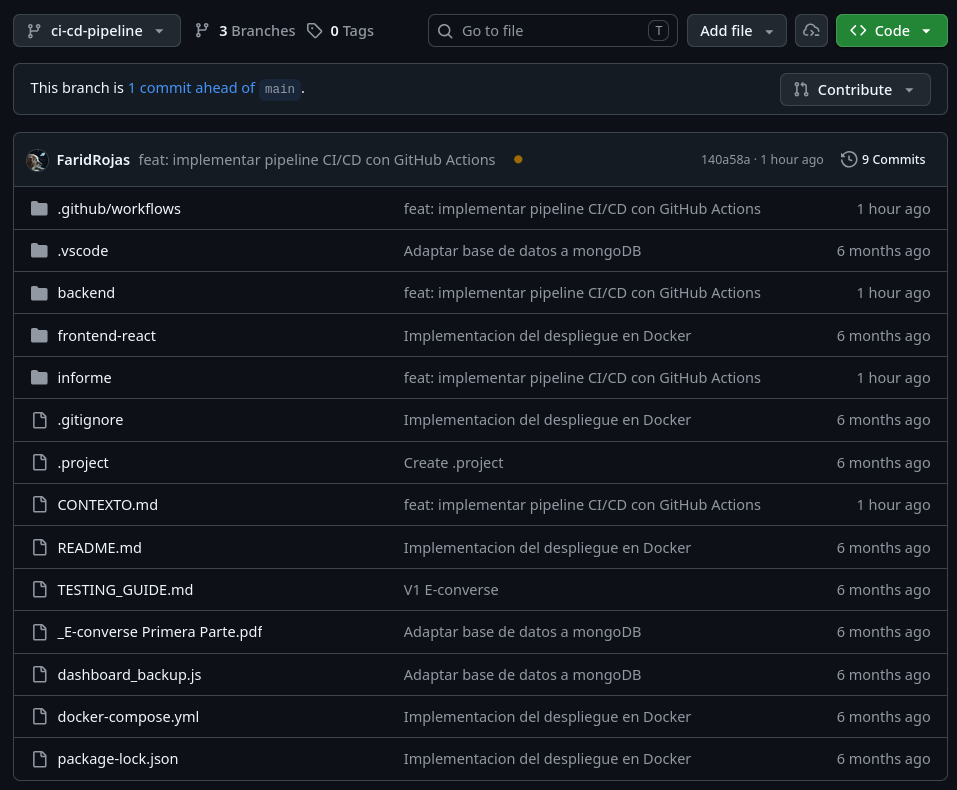
\includegraphics[width=0.55\textwidth]{Imagenes/estructura_repo.png}
    \caption{Estructura del repositorio en GitHub}
    \label{fig:estructura}
\end{figure}

% ============================================================
\section{Conceptos fundamentales de CI/CD}

\subsection{Integración Continua (CI)}
La Integración Continua es la práctica de fusionar frecuentemente los cambios de código de todos los desarrolladores en una rama compartida. Cada fusión activa un proceso automatizado que compila el código y ejecuta pruebas para detectar errores tempranamente.

\subsection{Entrega Continua (CD)}
La Entrega Continua extiende la CI automatizando el despliegue del software en entornos de prueba o producción. El objetivo es que cada cambio que pasa las pruebas esté listo para ser desplegado en cualquier momento.

\subsection{Conceptos de GitHub Actions}
\begin{itemize}
    \item \textbf{Workflow:} Proceso automatizado definido en un archivo YAML dentro de \texttt{.github/workflows/}. Se activa por eventos como \texttt{push} o \texttt{pull\_request}.
    \item \textbf{Job:} Conjunto de pasos (steps) que se ejecutan en un mismo runner. Los jobs pueden ejecutarse en paralelo o secuencialmente usando dependencias.
    \item \textbf{Step:} Acción individual dentro de un job. Puede ser un comando shell o una acción predefinida.
    \item \textbf{Runner:} Máquina virtual donde se ejecutan los jobs. GitHub proporciona runners con Ubuntu, Windows y macOS.
    \item \textbf{Artifact:} Archivo generado durante la ejecución del workflow que puede ser descargado o utilizado por otros jobs.
    \item \textbf{Secret:} Variable cifrada almacenada en la configuración del repositorio para proteger credenciales sensibles.
\end{itemize}

% ============================================================
\section{Estrategia de Branching}

Para este proyecto se utilizó una estrategia basada en \textbf{GitHub Flow}, creando una rama específica \texttt{ci-cd-pipeline} desde \texttt{main} para todo el desarrollo del pipeline. Esto permite:

\begin{itemize}
    \item No alterar la rama principal durante el desarrollo.
    \item Activar el pipeline automáticamente ante cada push a la rama.
    \item Facilitar la revisión mediante Pull Requests antes de integrar a \texttt{main}.
\end{itemize}

\begin{lstlisting}[style=bashstyle]
# Crear la rama de trabajo
git checkout -b ci-cd-pipeline

# Trabajar en la rama
git add .
git commit -m "feat: implementar pipeline CI/CD"
git push origin ci-cd-pipeline
\end{lstlisting}

\begin{figure}[H]
    \centering
    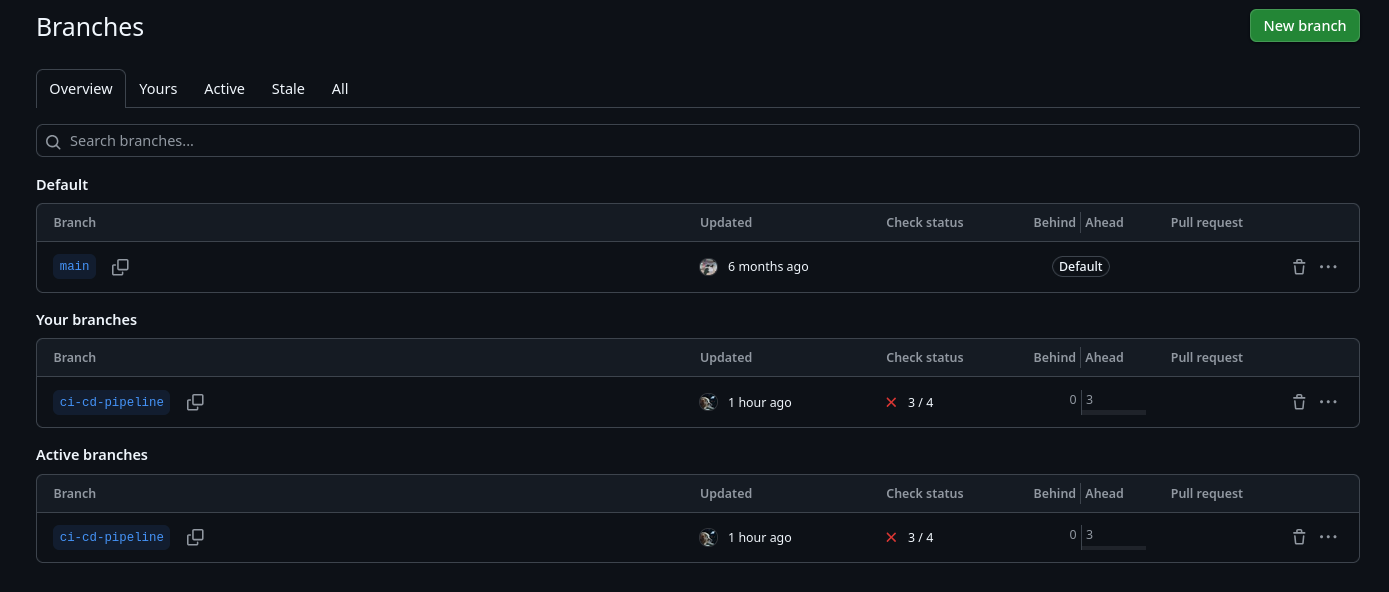
\includegraphics[width=0.85\textwidth]{Imagenes/branching_strategy.png}
    \caption{Estrategia de branching utilizada}
    \label{fig:branching}
\end{figure}

% ============================================================
\section{Explicación del Pipeline CI/CD}

El pipeline se compone de \textbf{4 jobs secuenciales} definidos en el archivo 
\texttt{.github/workflows/ci-cd.yml}:

\begin{enumerate}
    \item \textbf{Build \& Test} — Compilar y ejecutar pruebas
    \item \textbf{Docker Build \& Push} — Construir y subir imágenes Docker
    \item \textbf{Deploy} — Desplegar en servidor remoto via SSH
    \item \textbf{Notify} — Notificar resultado por email
\end{enumerate}

% ---- Job 1 ----
\subsection{Job 1: Build \& Test}

Este job se encarga de compilar tanto el backend como el frontend y ejecutar las pruebas unitarias del backend.

\textbf{Pasos principales:}
\begin{enumerate}
    \item Clonar el repositorio usando \texttt{actions/checkout@v4}
    \item Configurar JDK 17 con \texttt{actions/setup-java@v4} y cache de Maven
    \item Compilar el backend: \texttt{./mvnw -B clean compile}
    \item Ejecutar pruebas unitarias: \texttt{./mvnw -B test}
    \item Empaquetar JAR: \texttt{./mvnw -B package -DskipTests}
    \item Subir artefacto JAR con \texttt{actions/upload-artifact@v4}
    \item Configurar Node.js 20 e instalar dependencias del frontend
    \item Ejecutar lint y build del frontend con Vite
\end{enumerate}

\begin{figure}[H]
    \centering
    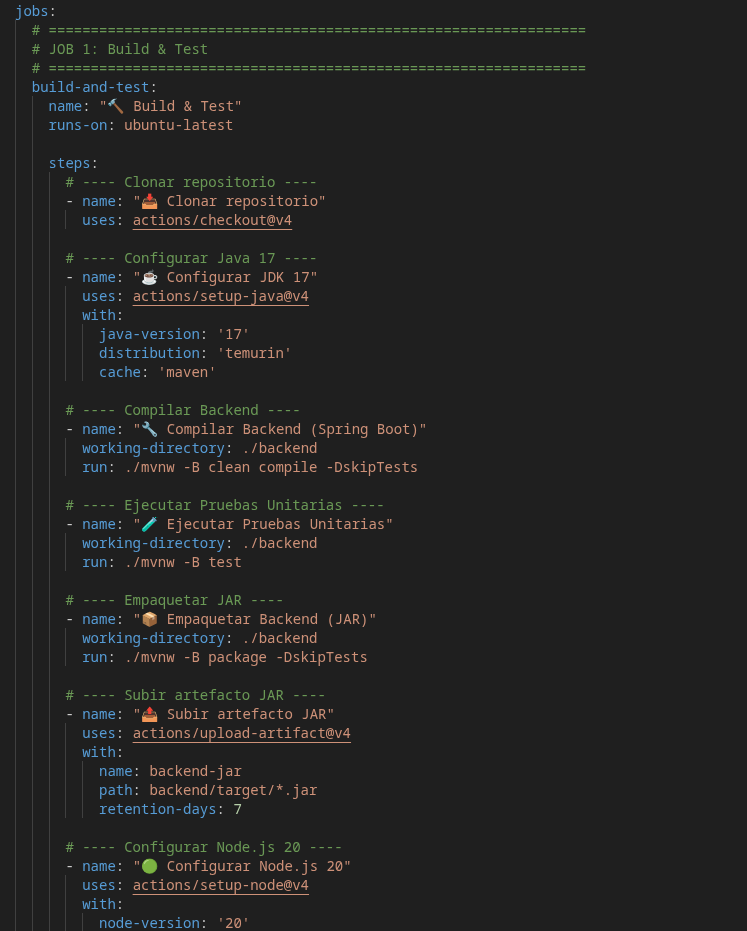
\includegraphics[width=0.95\textwidth]{Imagenes/workflow_build_test.png}
    \caption{Configuración del Job Build \& Test en el workflow YAML}
    \label{fig:build_test}
\end{figure}


% ---- Job 2 ----
\subsection{Job 2: Docker Build \& Push}

Una vez que el Job 1 finaliza exitosamente, este job construye las imágenes Docker del backend y frontend, y las sube a Docker Hub.

\textbf{Características:}
\begin{itemize}
    \item Login a Docker Hub usando secretos (\texttt{DOCKERHUB\_TOKEN})
    \item Docker Buildx para builds optimizados con cache
    \item Multi-stage builds: compilación separada del runtime
    \item Doble etiquetado: \texttt{latest} y SHA del commit
\end{itemize}

\begin{lstlisting}[style=yamlstyle]
# Etiquetas generadas para cada imagen
lyoks/e-converse-backend:latest
lyoks/e-converse-backend:<sha-del-commit>
lyoks/e-converse-frontend:latest
lyoks/e-converse-frontend:<sha-del-commit>
\end{lstlisting}

\begin{figure}[H]
    \centering
    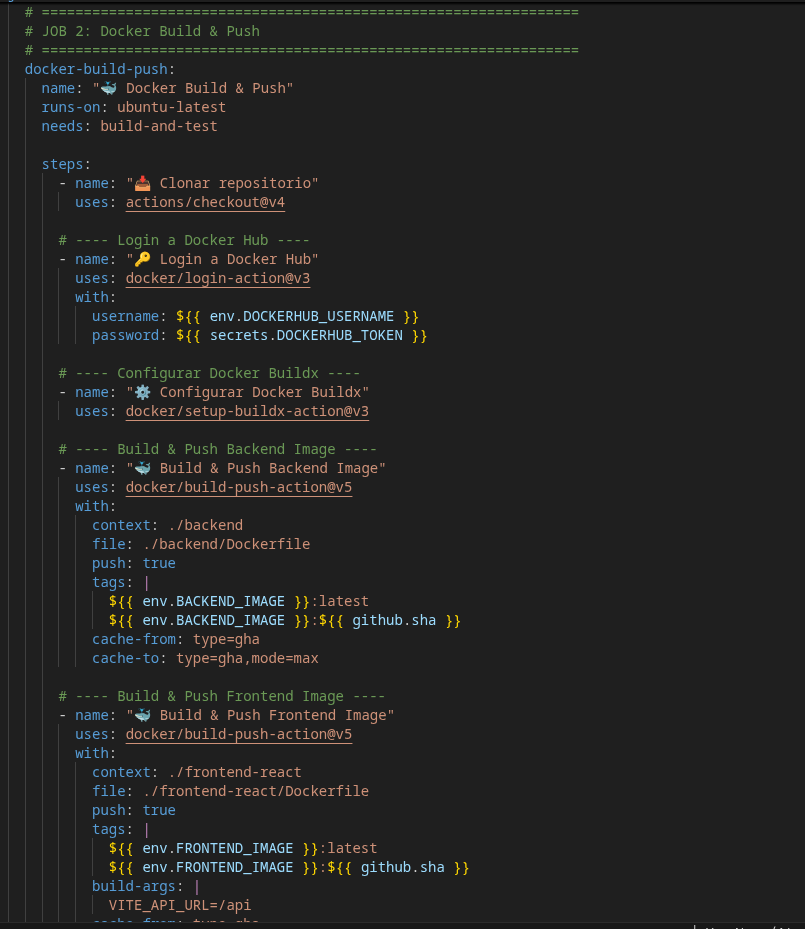
\includegraphics[width=0.95\textwidth]{Imagenes/workflow_docker_push.png}
    \caption{Configuración del Job Docker Build \& Push}
    \label{fig:docker_push}
\end{figure}


% ---- Job 3 ----
\subsection{Job 3: Deploy}

Este job despliega la aplicación en un servidor remoto (máquina virtual) mediante SSH. Utiliza la acción \texttt{appleboy/ssh-action@v1} para conectarse al servidor y ejecutar comandos Docker.

\textbf{Proceso de despliegue:}
\begin{enumerate}
    \item Conectar al servidor vía SSH con credenciales almacenadas en secretos
    \item Crear/actualizar el archivo \texttt{docker-compose.yml} en el servidor
    \item Descargar las imágenes más recientes (\texttt{docker pull})
    \item Detener los contenedores anteriores (\texttt{docker compose down})
    \item Levantar los nuevos contenedores (\texttt{docker compose up -d})
    \item Verificar el estado de los contenedores
\end{enumerate}

\begin{figure}[H]
    \centering
    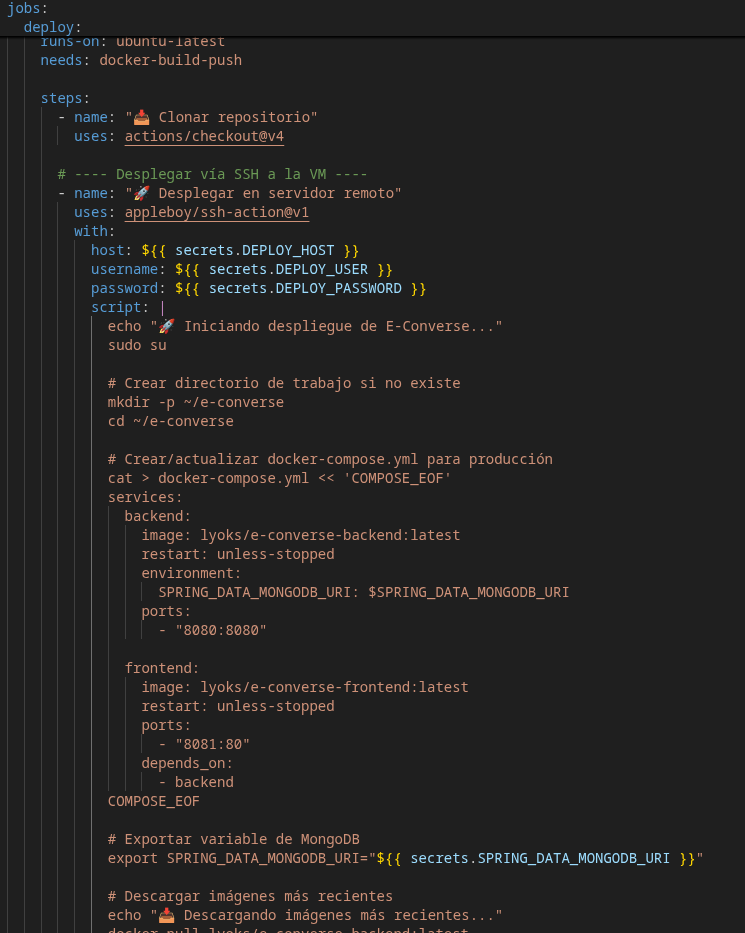
\includegraphics[width=0.95\textwidth]{Imagenes/workflow_deploy.png}
    \caption{Configuración del Job Deploy vía SSH}
    \label{fig:deploy}
\end{figure}


% ---- Job 4 ----
\subsection{Job 4: Notificaciones}

El último job envía una notificación por correo electrónico informando el resultado de cada etapa del pipeline. Se ejecuta \textbf{siempre} (con \texttt{if: always()}), independientemente de si los jobs anteriores fueron exitosos o fallaron.

\textbf{Información incluida en el correo:}
\begin{itemize}
    \item Repositorio, rama y commit
    \item Estado de cada job (éxito/fallo)
    \item Mensaje del commit
    \item Enlace directo a la ejecución en GitHub Actions
    \item Nombres de las imágenes Docker generadas
\end{itemize}

\begin{figure}[H]
    \centering
    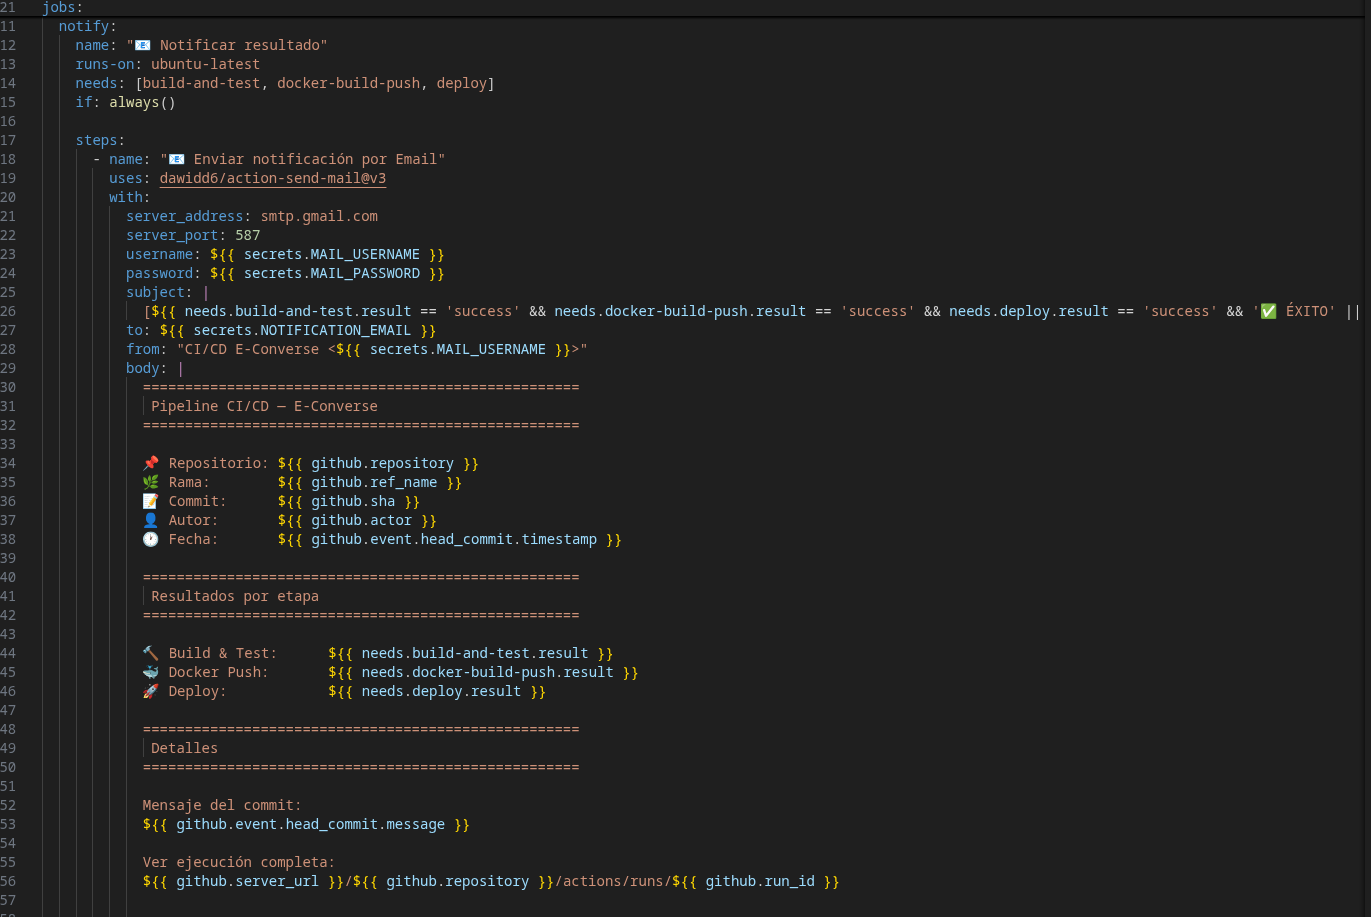
\includegraphics[width=0.95\textwidth]{Imagenes/workflow_notify.png}
    \caption{Configuración del Job de notificación por email}
    \label{fig:notify}
\end{figure}

% ============================================================
\section{Pruebas unitarias implementadas}

Se crearon pruebas unitarias para validar la lógica de negocio del backend usando \textbf{JUnit 5} y \textbf{Mockito}. Las pruebas mockean los repositorios de MongoDB para ejecutarse sin necesidad de una base de datos real.

\subsection{Pruebas del ProductoService}
\begin{itemize}
    \item Listar todos los productos
    \item Crear producto con y sin categoría
    \item Buscar producto por ID existente e inexistente
    \item Eliminar producto
    \item Verificación de precio y stock
\end{itemize}

\subsection{Pruebas del CategoriaService}
\begin{itemize}
    \item Listar todas las categorías
    \item Crear nueva categoría
    \item Buscar categoría por ID
    \item Eliminar categoría
    \item Actualizar categoría existente
\end{itemize}

\subsection{Pruebas del UsuarioService}
\begin{itemize}
    \item Listar usuarios con roles
    \item Crear usuario con contraseña encriptada (BCrypt)
    \item Buscar usuario por ID
    \item Actualizar usuario sin re-encriptar contraseña
    \item Eliminar usuario
\end{itemize}

\subsection{Pruebas del JwtTokenUtil}
\begin{itemize}
    \item Generar token JWT válido (estructura de 3 partes)
    \item Extraer username del token
    \item Validar token con usuario correcto e incorrecto
    \item Manejo de tokens malformados e inválidos
    \item Tokens diferentes para diferentes usuarios
\end{itemize}

\subsection{Pruebas del modelo Producto}
\begin{itemize}
    \item Constructor vacío y constructor completo
    \item Getters y setters de todos los campos
    \item Manejo de precios con decimales
    \item Manejo de stock cero
\end{itemize}

\begin{figure}[H]
    \centering
    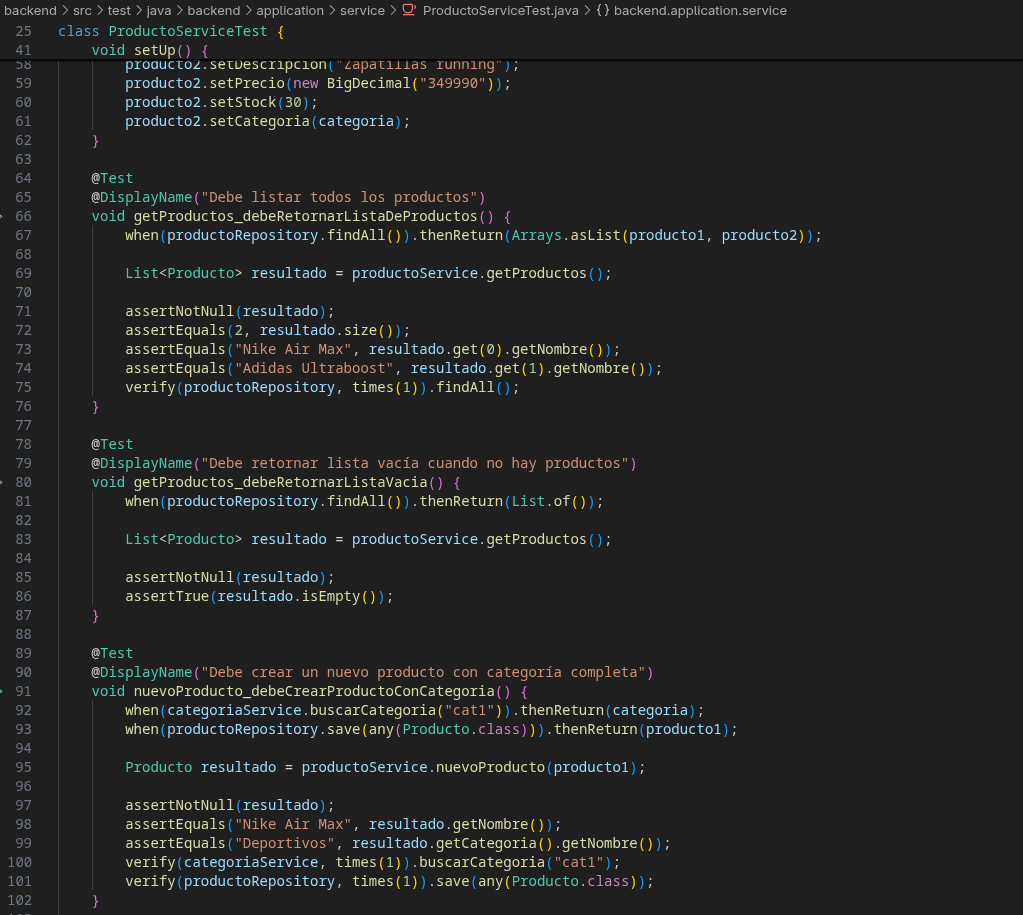
\includegraphics[width=0.95\textwidth]{Imagenes/tests_code.png}
    \caption{Ejemplo de código de pruebas unitarias (ProductoServiceTest)}
    \label{fig:tests_code}
\end{figure}

% ============================================================
\section{Gestión de secretos}

GitHub Actions provee un mecanismo seguro para almacenar credenciales sensibles mediante \textbf{Repository Secrets}. Los secretos se configuran en \texttt{Settings $\rightarrow$ Secrets and variables $\rightarrow$ Actions} del repositorio.

\subsection{Secretos configurados}

\begin{table}[H]
\centering
\begin{tabularx}{\textwidth}{|l|X|}
\hline
\textbf{Secreto} & \textbf{Descripción} \\
\hline
\texttt{DOCKERHUB\_TOKEN} & Token de acceso a Docker Hub para push de imágenes \\
\hline
\texttt{SPRING\_DATA\_MONGODB\_URI} & URI de conexión a MongoDB Atlas \\
\hline
\texttt{DEPLOY\_HOST} & IP del servidor de despliegue \\
\hline
\texttt{DEPLOY\_USER} & Usuario SSH del servidor \\
\hline
\texttt{DEPLOY\_PASSWORD} & Contraseña SSH del servidor \\
\hline
\texttt{MAIL\_USERNAME} & Email remitente (Gmail) para notificaciones \\
\hline
\texttt{MAIL\_PASSWORD} & Contraseña de aplicación de Gmail \\
\hline
\texttt{NOTIFICATION\_EMAIL} & Email destinatario de las notificaciones \\
\hline
\end{tabularx}
\caption{Secretos configurados en GitHub Actions}
\label{tab:secrets}
\end{table}

\textbf{Características de seguridad:}
\begin{itemize}
    \item Los secretos se cifran antes de almacenarse en GitHub
    \item No se imprimen en los logs de ejecución (se enmascaran con \texttt{***})
    \item Solo están disponibles para los workflows del repositorio
    \item Se referencian con la sintaxis \texttt{\$\{\{ secrets.NOMBRE \}\}}
\end{itemize}

\begin{figure}[H]
    \centering
    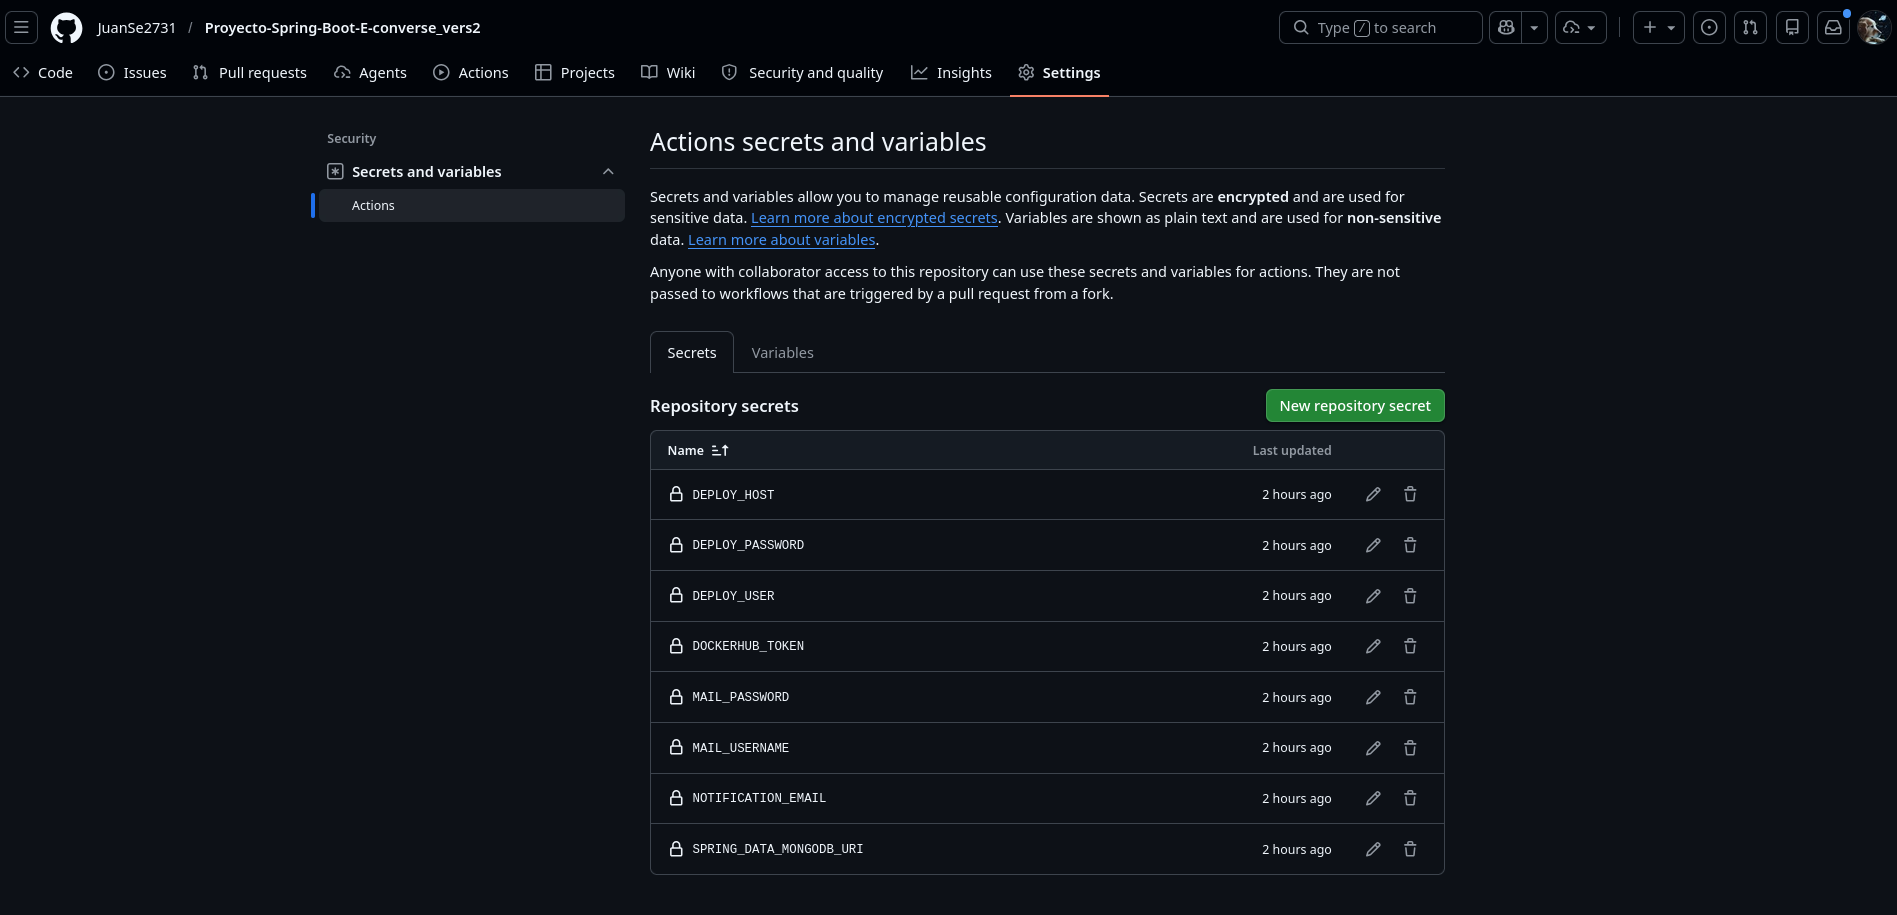
\includegraphics[width=0.85\textwidth]{Imagenes/github_secrets.png}
    \caption{Secretos configurados en el repositorio de GitHub}
    \label{fig:secrets}
\end{figure}

% ============================================================
\section{Registro de contenedores (Docker Hub)}

Las imágenes Docker se publican en \textbf{Docker Hub} bajo el usuario \texttt{lyoks}. Se utilizan dos repositorios de imágenes:

\begin{itemize}
    \item \texttt{lyoks/e-converse-backend} — Imagen del backend (Spring Boot + JRE 17)
    \item \texttt{lyoks/e-converse-frontend} — Imagen del frontend (Nginx + archivos estáticos)
\end{itemize}

\subsection{Estrategia de etiquetado}
Cada build genera dos tags:
\begin{itemize}
    \item \texttt{latest} — Siempre apunta a la versión más reciente
    \item \texttt{<sha>} — Tag inmutable con el SHA del commit, permite trazabilidad
\end{itemize}

\subsection{Dockerfiles (Multi-stage builds)}

\textbf{Backend:} Se utiliza un build en dos etapas: la primera compila el proyecto con Maven y la segunda ejecuta el JAR en un JRE mínimo.

\begin{figure}[H]
    \centering
    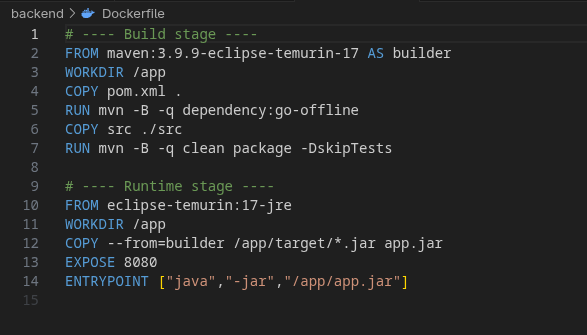
\includegraphics[width=0.85\textwidth]{Imagenes/dockerfile_backend.png}
    \caption{Dockerfile del Backend (multi-stage build)}
    \label{fig:dockerfile_backend}
\end{figure}

\textbf{Frontend:} Se compila el proyecto con Node.js/Vite y se sirve con Nginx Alpine.

\begin{figure}[H]
    \centering
    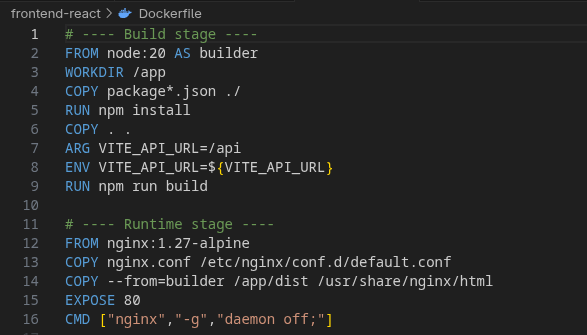
\includegraphics[width=0.85\textwidth]{Imagenes/dockerfile_frontend.png}
    \caption{Dockerfile del Frontend (multi-stage build)}
    \label{fig:dockerfile_frontend}
\end{figure}

\begin{figure}[H]
    \centering
    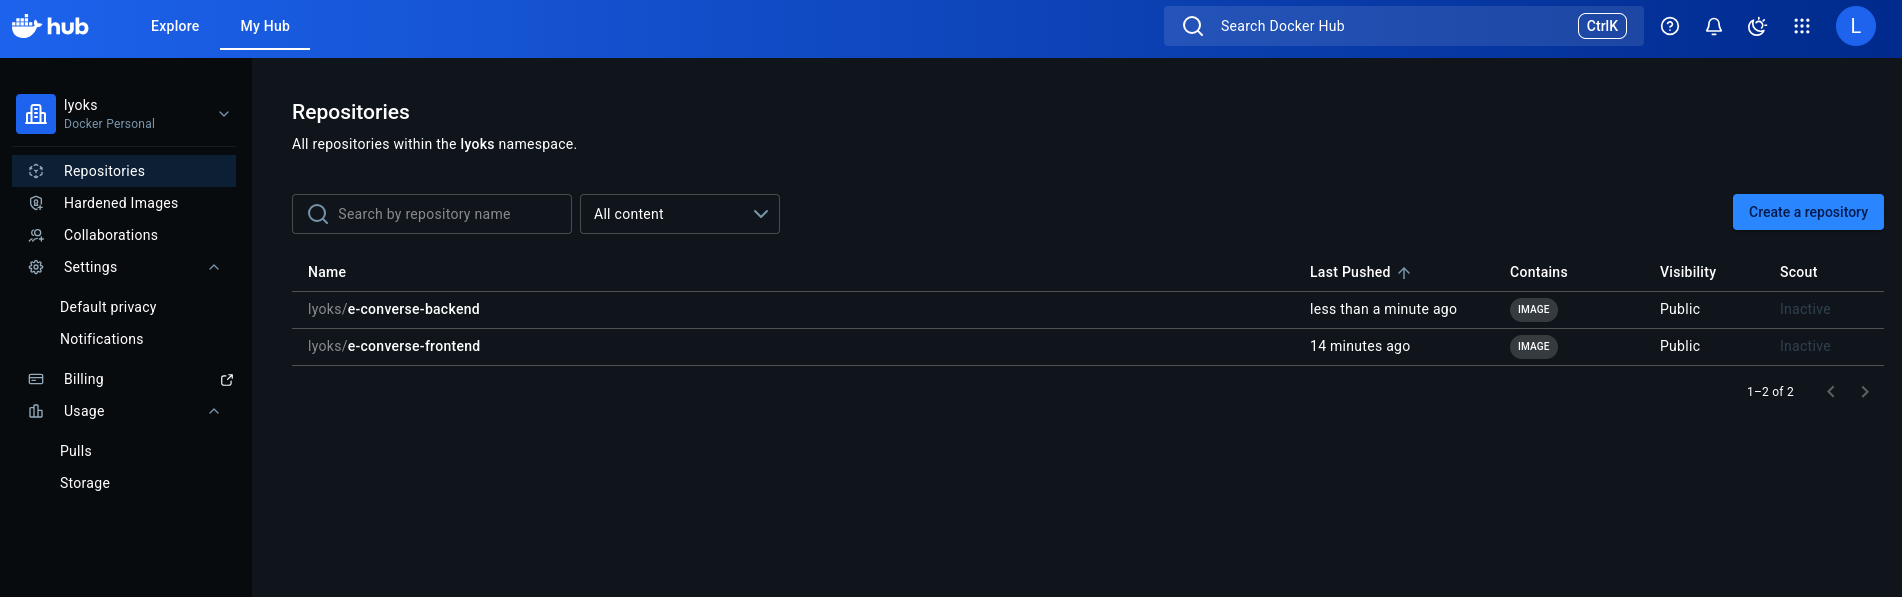
\includegraphics[width=0.85\textwidth]{Imagenes/dockerhub_repos.png}
    \caption{Repositorios de imágenes en Docker Hub}
    \label{fig:dockerhub_repos}
\end{figure}

% ============================================================
\section{Resultados obtenidos}

\subsection{Ejecución del pipeline completo}

\begin{figure}[H]
    \centering
    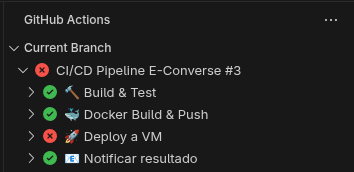
\includegraphics[width=0.95\textwidth]{Imagenes/pipeline_completo.png}
    \caption{Pipeline completo ejecutado en GitHub Actions}
    \label{fig:pipeline_completo}
\end{figure}

\subsection{Detalle de cada job}

\begin{figure}[H]
    \centering
    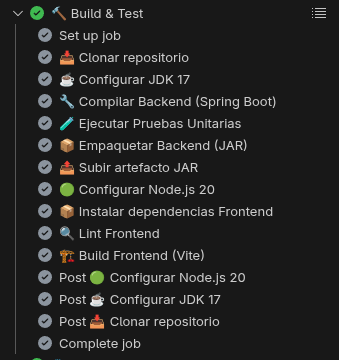
\includegraphics[width=0.95\textwidth]{Imagenes/job_build_detail.png}
    \caption{Detalle del Job Build \& Test}
    \label{fig:job_build}
\end{figure}

\begin{figure}[H]
    \centering
    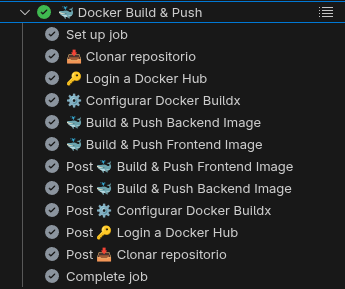
\includegraphics[width=0.95\textwidth]{Imagenes/job_docker_detail.png}
    \caption{Detalle del Job Docker Build \& Push}
    \label{fig:job_docker}
\end{figure}

\begin{figure}[H]
    \centering
    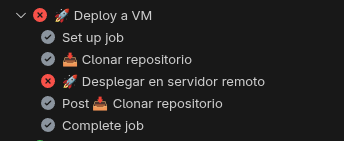
\includegraphics[width=0.95\textwidth]{Imagenes/job_deploy_detail.png}
    \caption{Detalle del Job Deploy}
    \label{fig:job_deploy}
\end{figure}

\begin{figure}[H]
    \centering
    
\includegraphics[width=0.95\textwidth]{Imagenes/job_notify_detail.png}
    \caption{Detalle del Job Notify}
    \label{fig:job_notify}
\end{figure}

\subsection{Notificación recibida}

\begin{figure}[H]
    \centering
    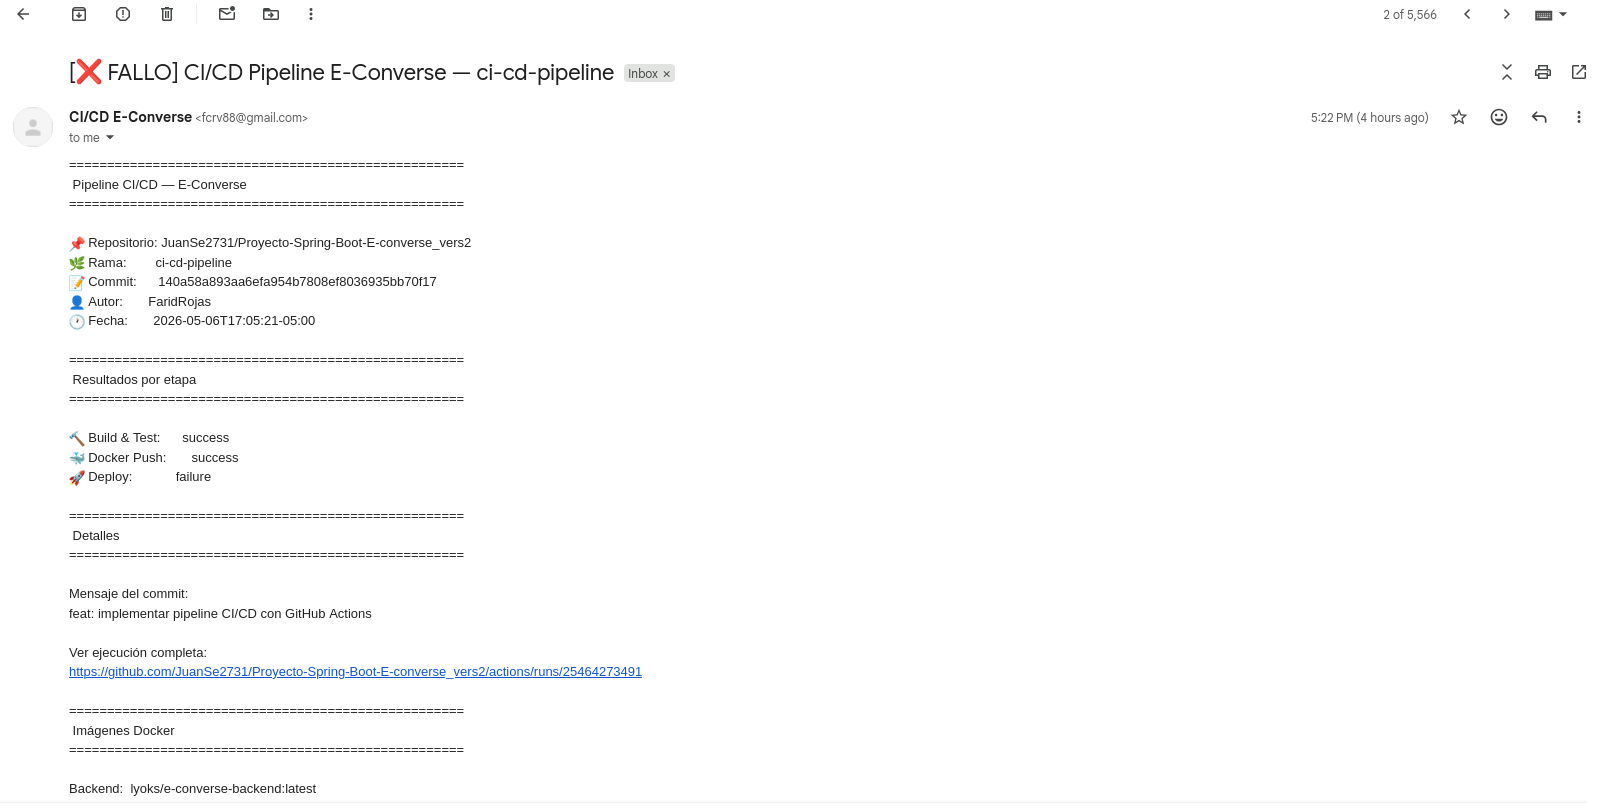
\includegraphics[width=0.85\textwidth]{Imagenes/email_notification.png}
    \caption{Correo de notificación recibido}
    \label{fig:email_notification}
\end{figure}

% ============================================================
\section{Análisis y conclusiones}

\subsection{Beneficios del CI/CD implementado}
\begin{itemize}
    \item \textbf{Automatización completa:} Desde el commit hasta el despliegue, sin intervención manual.
    \item \textbf{Detección temprana de errores:} Las pruebas unitarias se ejecutan en cada push, evitando que código defectuoso llegue a producción.
    \item \textbf{Trazabilidad:} El etiquetado de imágenes con SHA permite rastrear exactamente qué commit está desplegado.
    \item \textbf{Seguridad:} Los secretos se gestionan de forma cifrada mediante GitHub Secrets.
    \item \textbf{Visibilidad:} Las notificaciones por email mantienen al equipo informado del estado del pipeline.
    \item \textbf{Reproducibilidad:} El uso de Docker garantiza que la aplicación se ejecute de forma idéntica en cualquier entorno.
\end{itemize}

\subsection{Lecciones aprendidas}
\begin{itemize}
    \item La configuración de secretos en GitHub Actions es fundamental para proteger credenciales sensibles.
    \item Los multi-stage builds de Docker reducen significativamente el tamaño de las imágenes finales.
    \item La estrategia de branching (GitHub Flow) facilita la integración del pipeline con el flujo de desarrollo.
    \item Las notificaciones por email permiten reaccionar rápidamente ante fallos en el pipeline.
    \item Hay que tener en cuenta que Github Actions no es un servicio self-hosted, por lo que no se puede ejecutar el despliegue en un servidor fuera de redes públicas.
\end{itemize}

\end{document}
